% !TeX spellcheck = fr_FR
\chapter{Chapitre 4 : Lignes et appariement par lignes}

\noindent Ce chapitre est une visite guidée de la couche \emph{lignes} : comment nous construisons une vue unifiée des lignes à partir de GTFS et HRDF, à quoi ressemblent les données, ce que disent les chiffres, et comment nous effectuons l'appariement basé sur les lignes entre les arrêts ATLAS et les nœuds OSM. Attendez-vous à des extraits de code concis, des graphiques parlants et des explications pragmatiques.

\section{Des flux bruts à un fichier unique de lignes}
\noindent Cette section approfondit la vue d'ensemble du Chapitre~1 ; nous répétons volontairement certains points clés pour la fluidité.
\subsection{Ce qu'est \texttt{atlas\_routes\_unified.csv}}
Nous consolidons des \emph{signaux de ligne} issus de deux sources dans un seul fichier tabulaire :
\begin{itemize}
  \item \textbf{GTFS} (transport public) : identifiants de ligne, noms court/long, et la direction (0/1). Les directions sont dérivées via une heuristique \emph{premier$\rightarrow$dernier} par trajet, agrégée au niveau de la ligne.
  \item \textbf{HRDF} (horaire ferroviaire) : noms de lignes et chaînes de direction construites comme \emph{première gare$\rightarrow$dernière gare}, à la fois par noms et par paires de codes UIC.
\end{itemize}
Chaque ligne du CSV décrit « un signal de ligne pour un arrêt » :
\begin{center}
\small
\begin{tabular}{l l}
\toprule
Colonne & Signification \\
\midrule
\texttt{sloid} & Identifiant d'arrêt ATLAS\\
\texttt{source} & \texttt{gtfs} ou \texttt{hrdf}\\
\texttt{evidence} & Méthode d'inférence (p. ex. \texttt{gtfs\_first\_last}, \texttt{hrdf\_fplan})\\
\texttt{as\_of} & Date d'extraction\\
\texttt{route\_id}, \texttt{route\_id\_normalized} & ID GTFS brut et normalisé par année\\
\texttt{route\_name\_short}, \texttt{route\_name\_long} & Noms de ligne GTFS\\
\texttt{line\_name} & Ligne HRDF (si disponible)\\
\texttt{direction\_id} & Direction GTFS 0/1 (chaîne)\\
\texttt{direction\_name}, \texttt{direction\_uic} & Chaînes premier$\rightarrow$dernier humaines et UIC\\
\bottomrule
\end{tabular}
\end{center}
Cette structure est produite directement par l'écriture unifiée. La \textbf{normalisation par année} supprime les suffixes saisonniers (p. ex. \texttt{-j24}) pour stabiliser la comparaison inter-années :

\begin{codebox}[language=Python]{Normalisation des identifiants de ligne}
import re
def normalize_route_id(route_id: str) -> str:
    return re.sub(r"-j\\d+", "-jXX", route_id)
\end{codebox}

\subsection{Comment on le génère (vue d'ensemble)}
À haut niveau (voir \texttt{get\_atlas\_data.py}) :
\begin{enumerate}
  \item Charger GTFS en flux et ne garder que les arrêts suisses (IDs commençant par \texttt{85}).
  \item Premier passage sur \texttt{stop\_times} : pour chaque \texttt{trip\_id}, collecter le premier et le dernier arrêt suisses ; joindre à \texttt{trips} et \texttt{routes} pour obtenir l'ID et les noms de ligne.
  \item Construire, par ligne, les chaînes de direction « nom du premier arrêt $\rightarrow$ nom du dernier arrêt » (dédupliquées).
  \item Second passage sur \texttt{stop\_times} : dédupliquer \((\texttt{stop\_id},\ \texttt{route\_id},\ \texttt{direction\_id})\).
  \item Mapper \texttt{stop\_id} GTFS vers \texttt{sloid} ATLAS (règle stricte puis repli sûr).
  \item Parser HRDF (\texttt{GLEISE\_LV95}, \texttt{FPLAN}, \texttt{BAHNHOF}) pour obtenir lignes et directions premier$\rightarrow$dernier par \texttt{sloid}.
  \item Écrire un unique CSV propre combinant les deux sources.
\end{enumerate}

\section{Ce que disent les données unifiées}
Les chiffres ci-dessous sont calculés avec les scripts sous \texttt{memoire/scripts\_used/chap4}. Les sorties sont archivées dans \texttt{memoire/data/processed/chap4/}.

\subsection*{Vue GTFS}
\begin{itemize}
  \item \textbf{SLOIDs avec lignes GTFS} : \textbf{34\,781}
  \item \textbf{Nombre moyen de lignes uniques par \texttt{sloid}} : \textbf{2,73} (médiane \textbf{2,00})
  \item \textbf{Nombre moyen de couples (ligne, direction) par \texttt{sloid}} : \textbf{4,39} (médiane \textbf{3,00})
  \item \textbf{Groupes dupliqués pour (\texttt{sloid}, route\_norm, direction)} : \textbf{96,96\%}
  \item \textbf{Même ligne+direction, plusieurs chaînes de direction} : \textbf{96,95\%} des groupes présentent plus d'une chaîne premier$\rightarrow$dernier (patrons d'exploitation hétérogènes)
\end{itemize}

\subsection*{Vue HRDF}
\begin{itemize}
  \item \textbf{SLOIDs avec lignes HRDF} : \textbf{28\,757}
  \item \textbf{Nombre moyen de lignes uniques par \texttt{sloid}} : \textbf{2,32} (médiane \textbf{2,00})
  \item \textbf{Directions distinctes par (\texttt{sloid}, line\_name)} : \textbf{2,67} par UIC et \textbf{2,67} par nom (médianes \textbf{2,00})
  \item \textbf{Queues longues} : plusieurs couples (\texttt{sloid}, ligne) affichent \textbf{30–40} paires UIC premier$\rightarrow$dernier distinctes (branches, demi-tours)
\end{itemize}

\paragraph{En deux mots.} \emph{GTFS} couvre un grand nombre d'arrêts avec plusieurs directions par ligne ; \emph{HRDF} confirme une forte variété de directions terminales pour certaines lignes (queues longues). Cela implique qu'une comparaison robuste doit gérer la multiplicité des directions, pas seulement des identifiants de ligne.

\section{Genève : vues cartographiques}
Nous traçons Genève en utilisant uniquement les fichiers locaux (aucun téléchargement) : \texttt{data/raw/osm\_data.xml}, \texttt{data/processed/atlas\_routes\_unified.csv}, et \texttt{data/raw/stops\_ATLAS.csv}.

\begin{figure}[H]
  \centering
  \begin{minipage}[b]{0.48\textwidth}
    \centering
    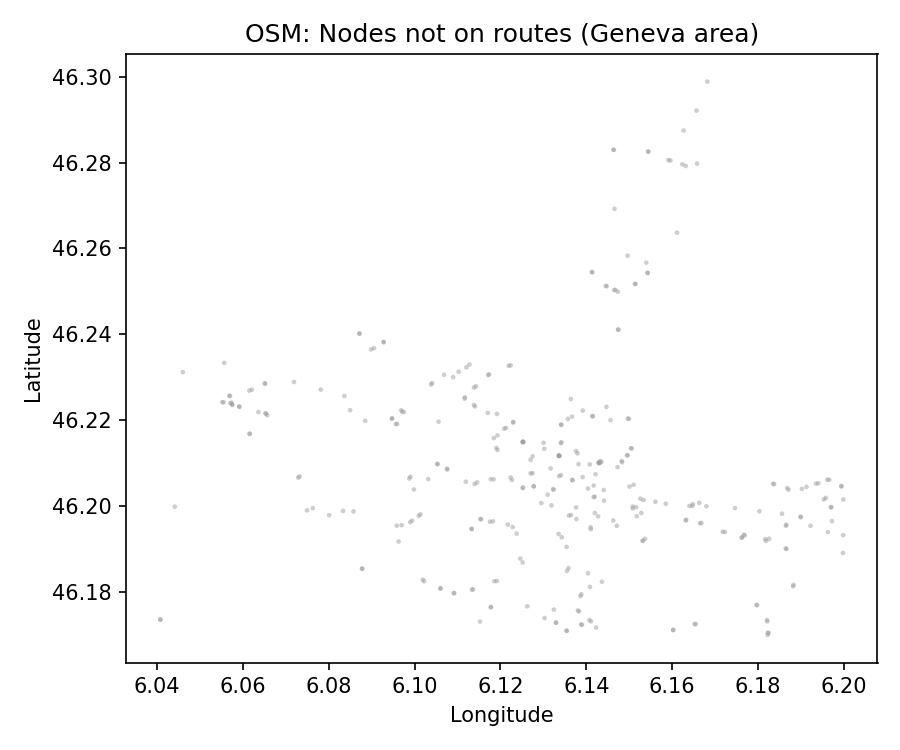
\includegraphics[width=\textwidth]{../figures/chap4/geneva_osm_non_routes_nodes.png}
    \caption*{OSM : nœuds ne faisant partie d\'\emph{aucune} relation de ligne (Genève).}
  \end{minipage}\hfill
  \begin{minipage}[b]{0.48\textwidth}
    \centering
    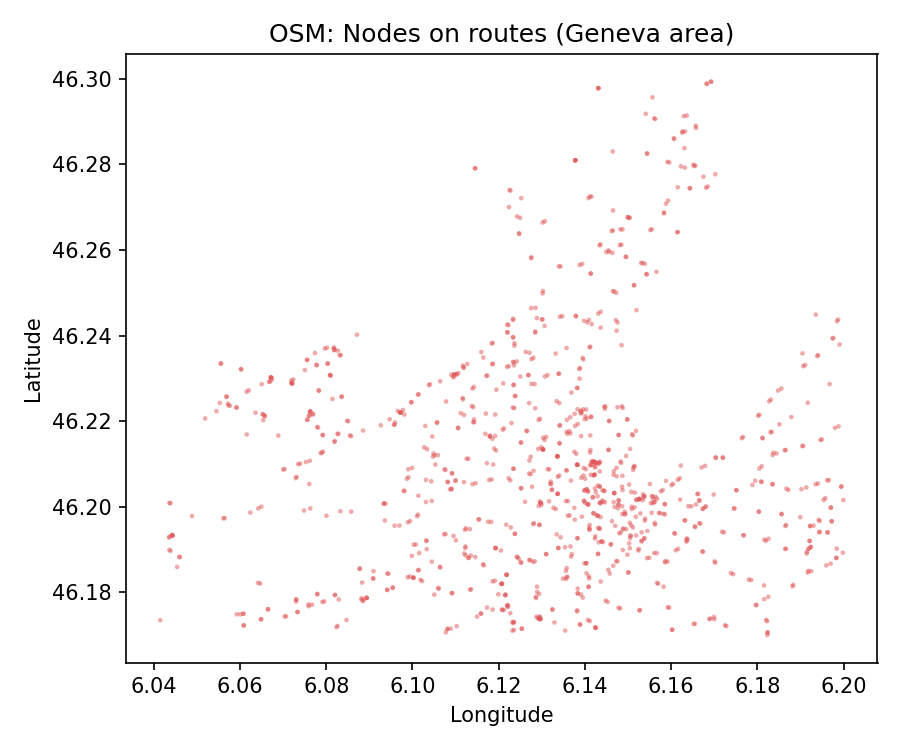
\includegraphics[width=\textwidth]{../figures/chap4/geneva_osm_routes_nodes.png}
    \caption*{OSM : nœuds participant à \emph{au moins une} relation de ligne (Genève).}
  \end{minipage}
  \caption{Nœuds OSM hors lignes vs. sur des lignes (région de Genève).}
\end{figure}

\begin{figure}[H]
  \centering
  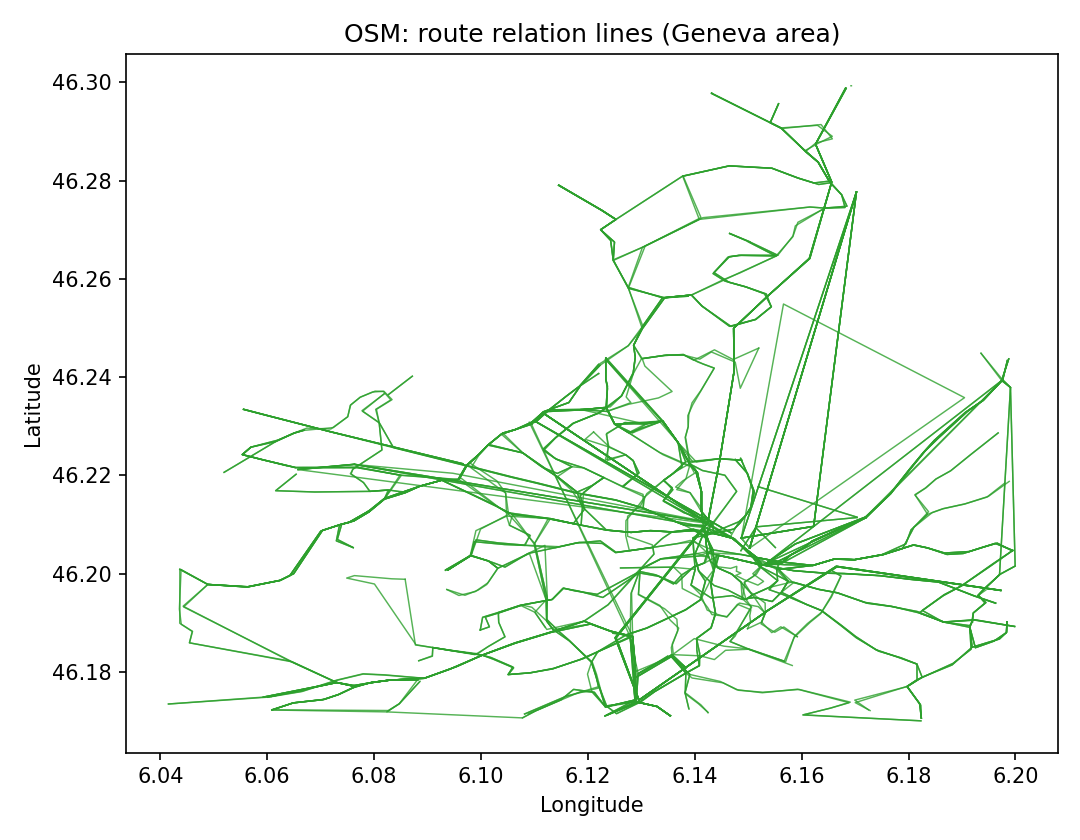
\includegraphics[width=0.8\textwidth]{../figures/chap4/geneva_osm_route_lines.png}
  \caption{OSM : tracé des lignes à partir des relations de type \texttt{route} (Genève). Géométrie bien structurée.}
\end{figure}

\begin{figure}[H]
  \centering
  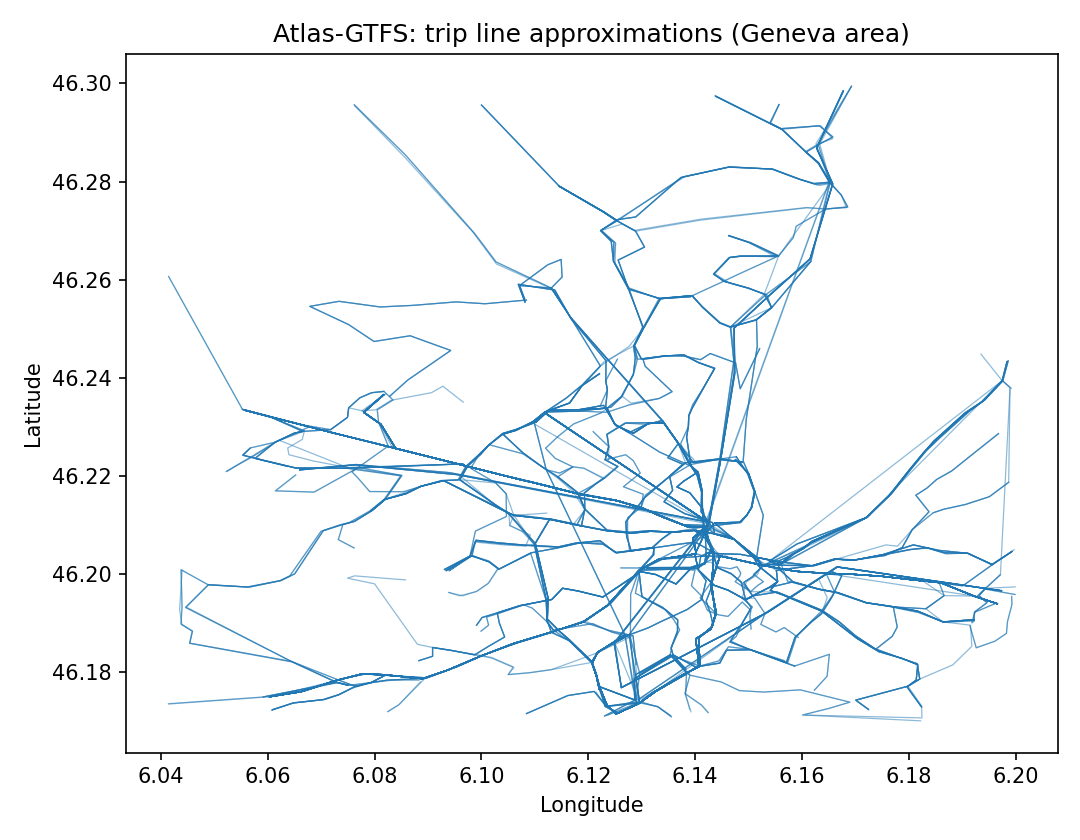
\includegraphics[width=0.8\textwidth]{../figures/chap4/geneva_atlas_gtfs_trip_lines.png}
  \caption{Atlas-GTFS : approximation des trajets (Genève). Lignes reconstruites depuis l'ordre des arrêts — plus fragmenté.}
\end{figure}

\begin{figure}[H]
  \centering
  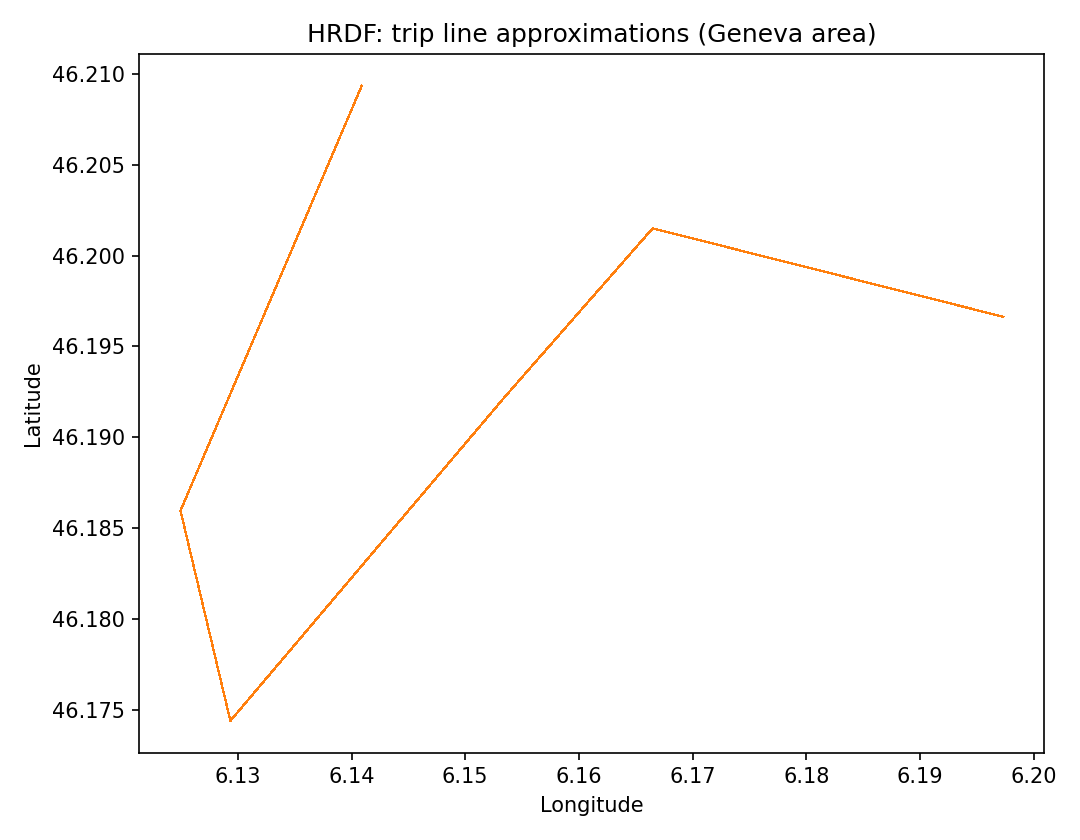
\includegraphics[width=0.8\textwidth]{../figures/chap4/geneva_hrdf_trip_lines.png}
  \caption{HRDF : approximation des trajets (Genève). Déduite des séquences \texttt{FPLAN} via les codes UIC.}
\end{figure}

\subsection*{Comment traçons-nous ces couches ?}
\textbf{OSM (routes)} : nous parcourons les relations \texttt{type=route}, récupérons la séquence de membres de type \texttt{node} (ou \texttt{way} si disponible) et relions leurs coordonnées lorsque le nœud se trouve dans la boîte Genève. Cela produit un \emph{linework} fidèle à la modélisation OSM.

\textbf{Atlas-GTFS (trajets)} : nous reconstruisons des polylignes en ordonnant les arrêts d'un trajet par \texttt{stop\_sequence} et en traçant les segments entre arrêts successifs, restreints à la boîte Genève. Pour éviter le fouillis, nous priorisons les séquences répétées (plus représentatives). Extrait en pseudo-code :

\begin{codebox}[language=Python]{Tracer les lignes \emph{Atlas-GTFS} (simplifié)}
stops = read_csv('stops.txt')[['stop_id','stop_lat','stop_lon']]
stop_times = read_csv('stop_times.txt')[['trip_id','stop_id','stop_sequence']]

# 1) Restreindre aux arrêts dans la boîte Genève
stops_ge = stops[in_bbox(stop_lat, stop_lon)]
stop_times_ge = stop_times[stop_id \in stops_ge.stop_id]

# 2) Reconstituer les séquences ordonnées par trajet
seq_map = {tid: tuple(g.sort_values('stop_sequence').stop_id)
           for tid, g in stop_times_ge.groupby('trip_id') if len(g) >= 2}

# 3) Compter les séquences répétées et en échantillonner
seq_counts = Counter(seq_map.values())
chosen = choose_top_sequences(seq_counts, max_trips=500)

# 4) Projeter en coordonnées et tracer
for seq in chosen:
    pts = [stops_ge.loc[id][('stop_lat','stop_lon')] for id in seq]
    draw_polyline(filter_in_bbox(pts))
\end{codebox}

\textbf{Atlas-HRDF (trajets)} : nous lisons \texttt{FPLAN}, détectons les séquences de gares (UIC), puis projetons celles dont au moins une gare est dans la boîte Genève via le couple \texttt{(UIC $\rightarrow$ coordonnée)} issu d'ATLAS. L'algorithme traite plus d'un million de trajets HRDF et sélectionne ceux traversant la région de Genève. Pour éviter les artéfacts visuels, nous segmentons les polylignes sur les grands sauts spatiaux (>3 km) et ne conservons que les segments ayant au moins 2 points dans la boîte. Le résultat final montre 500 segments de trajets ferroviaires réalistes pour la région genevoise.

\section{D'autres vues utiles}
\begin{figure}[H]
  \centering
  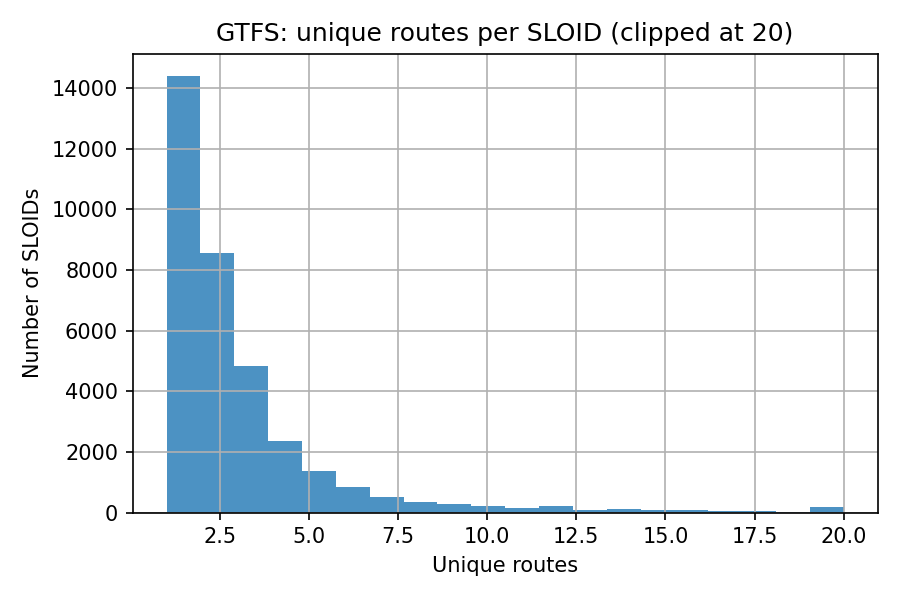
\includegraphics[width=0.75\textwidth]{../figures/chap4/hist_gtfs_routes_per_sloid.png}
  \caption{Distribution du nombre de lignes GTFS uniques par \texttt{sloid} (coupée à 20).}
\end{figure}

\begin{figure}[H]
  \centering
  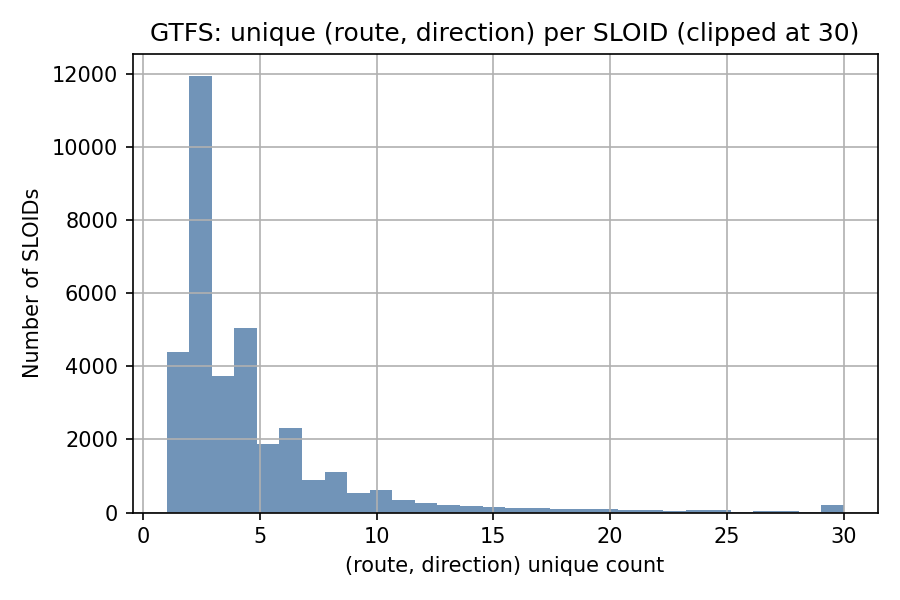
\includegraphics[width=0.75\textwidth]{../figures/chap4/hist_gtfs_route_dir_per_sloid.png}
  \caption{Distribution du nombre de couples (ligne, direction) par \texttt{sloid} (coupée à 30).}
\end{figure}

\begin{figure}[H]
  \centering
  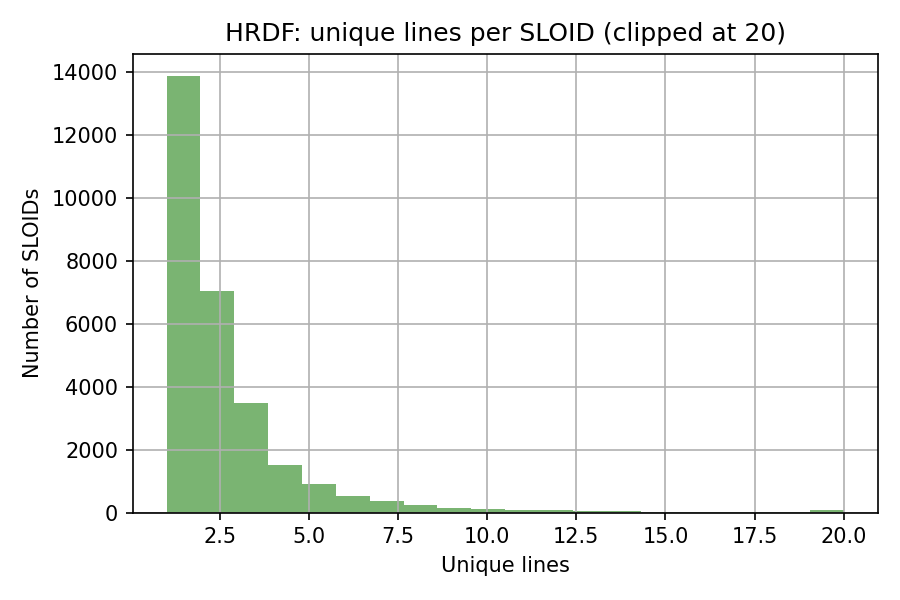
\includegraphics[width=0.75\textwidth]{../figures/chap4/hist_hrdf_lines_per_sloid.png}
  \caption{Distribution du nombre de lignes HRDF uniques par \texttt{sloid} (coupee a 20).}
\end{figure}

\paragraph{Ce que montrent les distributions.} Lors de la generation des graphiques, le script imprime un resume statistique sur le terminal :
\begin{itemize}
  \item \textbf{GTFS --- lignes par \texttt{sloid}} : moyenne \textbf{2,733}, mediane \textbf{2,0}, p10 \textbf{1}, p90 \textbf{5}, max \textbf{58}. \emph{Lecture} : la plupart des arrets ont 2--5 lignes, quelques hubs depassent largement.
  \item \textbf{GTFS --- (ligne, direction) par \texttt{sloid}} : moyenne \textbf{4,392}, mediane \textbf{3,0}, p10 \textbf{1}, p90 \textbf{8}, max \textbf{95}. \emph{Lecture} : les directions doublent naturellement la diversite par rapport aux seules lignes.
  \item \textbf{HRDF --- lignes par \texttt{sloid}} : moyenne \textbf{2,318}, mediane \textbf{2,0}, p10 \textbf{1}, p90 \textbf{4}, max \textbf{33}. \emph{Lecture} : structure comparable a GTFS, avec des extremes moins frequents.
\end{itemize}
Ces elements nous permettent de commenter les queues longues et la variabilite directionnelle dans le corps du texte, sans surcharge graphique.

\subsection*{Comment obtenons-nous les \emph{tokens} HRDF UIC ?}
Rappel synthetique (voir Chapitre~1) :
\begin{itemize}
  \item Depuis \texttt{GLEISE\_LV95} : \texttt{sloid} $\mapsto$ \texttt{UIC} et reference de quai (\texttt{\#ref}).
  \item Depuis \texttt{FPLAN} : pour les trajets traversant ces paires \((UIC,\ \#ref)\), on extrait la premiere et la derniere gare (codes UIC) et le nom de ligne (\texttt{*L}).
  \item Depuis \texttt{BAHNHOF} : on associe des noms aux UIC et on construit des chaines premier$\rightarrow$dernier par \emph{noms} et par \emph{UIC} (p. ex. \texttt{"Geneve $\rightarrow$ Lausanne"} et \texttt{"8501008 $\rightarrow$ 8501120"}).
\end{itemize}
Ces tokens \((\texttt{line\_name},\ \texttt{direction\_uic})\) sont compares aux chaines UIC premier$\rightarrow$dernier derivees d'OSM pour appuyer l'appariement au niveau HRDF lorsque les identifiants GTFS manquent dans OSM.

\section{Appariement par lignes : comment ça marche}
L'appariement compare les tokens de ligne connus pour un \texttt{sloid} ATLAS aux tokens derives des noeuds OSM a proximite (KD-tree, rayon configurable : \texttt{50 m} par defaut). Les tokens sont soit \textbf{GTFS} \((\texttt{route\_id},\ \texttt{direction\_id})\, avec normalisation eventuelle), soit \textbf{HRDF} \((\texttt{line\_name},\ \texttt{direction\_uic})\).

\subsection{Candidats par distance}
Nous tentons l'appariement en quatre paliers :
\begin{enumerate}
  \item \textbf{P1/P2 (tokens GTFS)} : intersection non vide entre les tokens GTFS du \texttt{sloid} et ceux d'un noeud candidat.
  \item \textbf{P3 (HRDF par UIC)} : presence d'une chaine UIC premier$\rightarrow$dernier du cote du noeud (membre d'une relation OSM) correspondant a une chaine HRDF du \texttt{sloid}.
  \item \textbf{P4 (repli par noms)} : concordance entre une chaine \emph{nominale} OSM premier$\rightarrow$dernier et une chaine unifiee (cote ATLAS).
\end{enumerate}
Extrait minimaliste de la logique des tokens :

\begin{codebox}[language=Python]{Intersection de tokens GTFS}
node_tokens = set()
for route in node_routes:
    rid = route.gtfs_route_id
    did = route.direction_id or '0'
    if rid:
        node_tokens.add((rid, did))
        rid_norm = normalize_route_id(rid)  # '-j25' -> '-jXX'
        if rid_norm:
            node_tokens.add((rid_norm, did))

if gtfs_tokens & node_tokens:
    match = ('gtfs', 'gtfs_tokens')
\end{codebox}

La normalisation des identifiants de ligne utilisée dans tout le système est :

\begin{codebox}[language=Python]{Normalisation \texttt{route\_id}}
import re

def normalize_route_id(route_id: str) -> str:
    return re.sub(r"-j\\d+", "-jXX", route_id)
\end{codebox}

\subsection{Paramètres}
\begin{itemize}
  \item \textbf{Rayon} : \texttt{50 m} par défaut. Plus petit $\Rightarrow$ moins de faux positifs, mais risque de manquer des arrêts légèrement décalés dans OSM.
  \item \textbf{Types de tokens} : activer uniquement GTFS ou inclure les paliers HRDF.
  \item \textbf{Normalisation} : comparer avec ou sans \texttt{-jXX}.
\end{itemize}

\section{Appariement par lignes : les chiffres}
Avec le script optimisé (\texttt{route\_matching\_stats.py}, exécuté sur les fichiers déjà présents), nous obtenons :
\begin{itemize}
  \item \textbf{Tokens GTFS} : \texttt{7\,252} ; \textbf{tokens OSM} : \texttt{7\,121} ; \textbf{chevauchement} : \texttt{3\,200} ; \textbf{Jaccard} : \textbf{0,2864}.
  \item \textbf{Couverture par \texttt{sloid} (GTFS)} : moyenne \textbf{2,64}, médiane \textbf{2}, p90 \textbf{6} ; au moins un token couvert pour \textbf{73,4\%} des \texttt{sloid}s.
  \item \textbf{Au niveau des lignes} : lignes GTFS uniques \textbf{3\,839} ; avec correspondance OSM \textbf{1\,664} $\Rightarrow$ \textbf{43,3\%} de lignes appariées.
  \item \textbf{Chaînes UIC premier$\rightarrow$dernier} : HRDF \textbf{8\,818}, OSM \textbf{5\,633}, chevauchement \textbf{2\,935}.
\end{itemize}
\noindent \emph{Lecture rapide} : la similarité \textbf{Jaccard $\approx 0{,}29$} indique un recouvrement substantiel mais non total des tokens GTFS dans OSM ; le taux d'appariement \textbf{43\%} au niveau des lignes confirme une couverture utile pour un appariement de haute précision.

\subsection{Efficacité de l'appariement par lignes : une analyse complète}
Pour quantifier l'efficacité réelle de l'appariement par lignes, nous avons mené une \textbf{analyse comparative} entre l'appariement exact seul et l'appariement par lignes seul sur l'ensemble complet des arrêts ATLAS. Cette évaluation révèle des insights cruciaux sur la valeur ajoutée et la complémentarité des deux méthodes.

\paragraph{Méthodologie.} L'étude compare deux pipelines isolés : (1) appariement exact basé uniquement sur les références UIC, et (2) appariement par lignes utilisant exclusivement les tokens de lignes GTFS et HRDF. Chaque méthode opère sur l'ensemble des 56\,515 arrêts ATLAS avec un rayon de 50 mètres.

\paragraph{Résultats quantitatifs.}
\begin{itemize}
  \item \textbf{Appariement exact} : \textbf{21\,250} paires arrêt$\leftrightarrow$nœud
  \item \textbf{Appariement par lignes} : \textbf{29\,582} paires arrêt$\leftrightarrow$nœud
  \item \textbf{Intersection} : \textbf{6\,971} paires communes aux deux méthodes
  \item \textbf{Similarité Jaccard} : \textbf{0,159} — faible recouvrement, forte complémentarité
  \item \textbf{Précision de l'appariement par lignes} : \textbf{23,6\%} des correspondances de lignes sont confirmées par l'appariement exact
  \item \textbf{Valeur ajoutée} : \textbf{40,0\%} des arrêts ATLAS obtiennent de nouvelles correspondances uniquement via les lignes
\end{itemize}

\paragraph{Qualité spatiale.} L'appariement par lignes maintient une précision spatiale élevée : distance moyenne de \textbf{11,9 m}, médiane \textbf{8,2 m}, et \textbf{86\%} des correspondances à moins de 25 mètres. Cette qualité spatiale démontre que les tokens de ligne, bien qu'indirects, identifient des nœuds OSM géographiquement cohérents.

\paragraph{Insights stratégiques.} L'analyse révèle une \textbf{complémentarité remarquable} : l'appariement par lignes trouve \textbf{22\,611} nouvelles paires que l'appariement exact ne détecte pas, soit un \textbf{facteur de complémentarité de 1,58}. Cela signifie que pour chaque correspondance manquée par l'appariement exact, l'appariement par lignes en propose environ 1,6 nouvelle.

Cette performance s'explique par la richesse des données de lignes (\textbf{34\,781} arrêts ATLAS avec données GTFS, \textbf{28\,757} avec HRDF) et la couverture étendue d'OSM (\textbf{51\,286} nœuds avec informations de lignes). L'appariement par lignes exploite ainsi des signaux de transport public que l'appariement exact, limité aux références UIC explicites, ne peut capturer.

\begin{figure}[H]
  \centering
  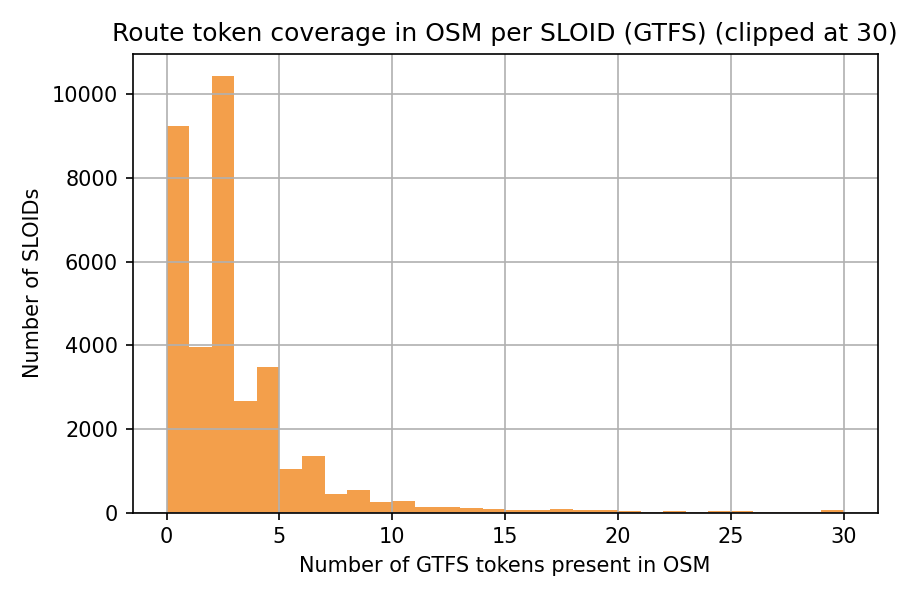
\includegraphics[width=0.75\textwidth]{../figures/chap4/hist_route_token_coverage_per_sloid.png}
  \caption{Nombre de tokens GTFS \((ligne, direction)\) par \texttt{sloid} retrouvés dans OSM (coupée à 30).}
\end{figure}

\section{Scripts utilisés dans ce chapitre}
Tous les scripts résident sous \texttt{memoire/scripts\_used/chap4} et n'opèrent que sur \texttt{data/raw} et \texttt{data/processed} :
\begin{itemize}
  \item \texttt{compute\_unified\_stats.py} : lit \texttt{atlas\_routes\_unified.csv}, produit des statistiques (avec impressions de distribution sur le terminal) et des histogrammes.
  \item \texttt{geneva\_maps.py} : génère les vues OSM et ATLAS (incluant désormais les nœuds OSM hors et sur relations de ligne).
  \item \texttt{geneva\_route\_lines.py} : trace les lignes OSM, \textbf{Atlas-GTFS} et HRDF (détection robuste de \texttt{FPLAN}, traitement de plus d'un million de trajets).
  \item \texttt{route\_matching\_stats.py} : calcule chevauchements et couvertures, avec logs de progression et un mode rapide.
  \item \texttt{route\_effectiveness\_analysis.py} : analyse comparative complète de l'efficacité de l'appariement par lignes vs. exact.
  \item \texttt{compare\_exact\_vs\_route.py} : comparaison directe des deux approches d'appariement pour quantifier la complémentarité.
\end{itemize}

\section{Bilan et perspectives}
\textbf{Atouts}. L'écriture unifiée offre une vue compacte et exploitable des lignes par arrêt, toutes sources confondues. Le pipeline d'appariement privilégie la précision (intersections de tokens) avec des seuils de distance conservateurs. La normalisation par année stabilise les comparaisons inter-versions.

\textbf{Complexités observées}.
\begin{itemize}
  \item \emph{Multiplicité des directions} : pour une même ligne+direction, des chaînes premier$\rightarrow$dernier multiples coexistent (branches, retournements).
  \item \emph{Taggage OSM partiel} : \texttt{gtfs:route\_id} est souvent présent, mais les indices de direction sont moins systématiques.
  \item \emph{Dérive spatiale} : de petits écarts géocodage/placement peuvent sortir un bon candidat d'un rayon trop strict en zones denses.
\end{itemize}

\textbf{Pistes d'amélioration}.
\begin{itemize}
  \item Cohérence par séquences : comparer de courts segments proches de l'arrêt à l'ordre GTFS pour désambigüiser les grappes denses.
  \item Score apprenable : combiner distance, tokens, similarité de noms, indices HRDF dans un \emph{ranker} entraîné sur des paires annotées.
  \item Robustesse directionnelle : distiller de nombreuses chaînes premier$\rightarrow$dernier en un petit ensemble de terminus canoniques par branche.
  \item Rafraîchissement incrémental : \emph{cacher} les sets de tokens par version et ne rematcher que les \texttt{sloid}s impactés.
  \item Optimisation multi-critères : développer des fonctions de coût intégrant qualité spatiale, couverture des tokens, et cohérence temporelle pour maximiser simultanément précision et rappel.
\end{itemize}

\noindent \textbf{En bref} : l'appariement par lignes ajoute un signal fort et indépendant qui complète les méthodes exactes/nominales/distance. L'analyse d'efficacité démontre sa valeur ajoutée substantielle (\textbf{40\%} de nouveaux appariements) tout en maintenant une qualité spatiale élevée (86\% des correspondances sous 25 m). Cette approche transforme les métadonnées de transport public en un levier puissant pour l'appariement géospatial, ouvrant la voie à des systèmes de correspondance plus robustes et complets.
